\documentclass[]{article}
\usepackage[letterpaper]{geometry}
\usepackage[utf8]{inputenc}
\usepackage{fancyhdr}
\usepackage{graphicx}
\usepackage{multicol} 

\geometry{headheight = 5 cm,
          left=2 cm,
          right=2 cm,
          top=4.35 cm}

\pagestyle{fancy}

\lhead{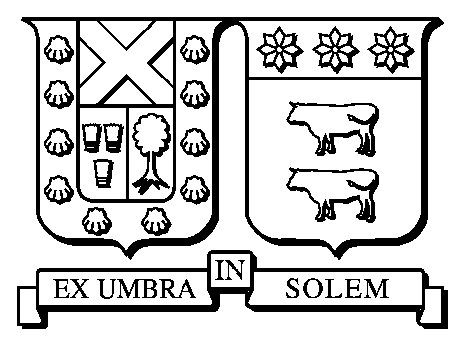
\includegraphics[height=1.5cm]{imagenes/isotipo}}
\rhead{\sc\small Universidad Técnica Federico Santa María\\Campus Santiago San Joaquín\\Optimización\\2$^\circ$ semestre 2017}

\cfoot{\thepage}

\renewcommand{\headrulewidth}{0pt}

\title{Laboratorio 3}

\author{Profesor: Carlos Castro\\ 
        Integrantes: Giorgio Pellizzari y Gabriel Valenzuela}
\date{Diciembre 2017}

\begin{document}

\maketitle
\thispagestyle{fancy}

\section{Pregunta 1:}

A continuación se procede a mostrar la red de precedencia a partir de los datos de la tabla 1:

\begin{figure}[ht] 
\centering
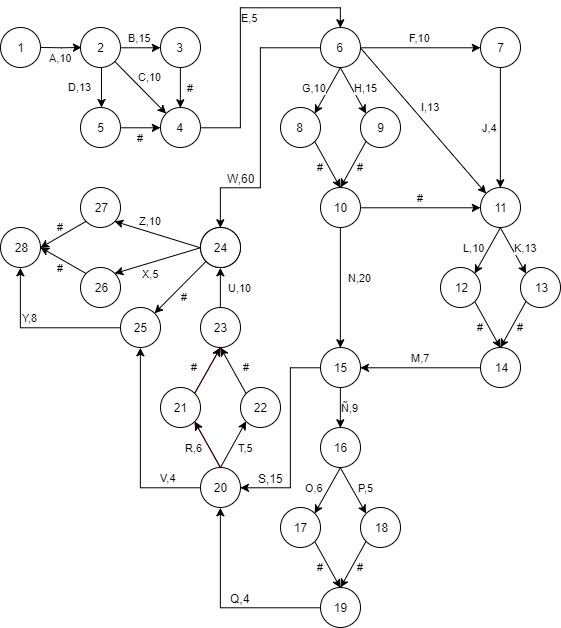
\includegraphics[scale=0.56]{imagenes/grafo.png}
\caption{Red de precedencia. Las actividades \# son actividades de tiempo nulo.}
\end{figure}

A continuación se presenta una tabla con los tiempos más tempranos y tardíos para cada actividad:

\begin{table}[ht]
\centering
\begin{tabular}{|c|c|c|c|c|}
\hline
Act. & E min & E max & L min & L max \\ \hline
A    & 0     & 10    & 0     & 10    \\ \hline
B    & 10    & 25    & 10    & 25    \\ \hline
C    & 10    & 20    & 15    & 25    \\ \hline
D    & 10    & 23    & 12    & 25    \\ \hline
E    & 25    & 30    & 25    & 30    \\ \hline
F    & 30    & 40    & 31    & 41    \\ \hline
G    & 30    & 40    & 35    & 45    \\ \hline
H    & 30    & 45    & 30    & 45    \\ \hline
I    & 30    & 43    & 32    & 45    \\ \hline
J    & 40    & 44    & 41    & 45    \\ \hline
K    & 45    & 58    & 45    & 58    \\ \hline
L    & 45    & 55    & 48    & 58    \\ \hline
M    & 58    & 65    & 58    & 65    \\ \hline
N    & 45    & 65    & 45    & 65    \\ \hline
Ñ    & 65    & 74    & 65    & 74    \\ \hline
O    & 74    & 80    & 74    & 80    \\ \hline
P    & 74    & 79    & 75    & 80    \\ \hline
Q    & 80    & 84    & 80    & 84    \\ \hline
R    & 84    & 90    & 84    & 90    \\ \hline
S    & 65    & 80    & 69    & 84    \\ \hline
T    & 84    & 89    & 85    & 90    \\ \hline
U    & 90    & 100   & 90    & 100   \\ \hline
V    & 84    & 88    & 98    & 102   \\ \hline
W    & 30    & 90    & 40    & 100   \\ \hline
X    & 100   & 105   & 105   & 110   \\ \hline
Y    & 100   & 108   & 102   & 110   \\ \hline
Z    & 100   & 110   & 100   & 110   \\ \hline
\end{tabular}
\end{table}

\newpage
Se encontraron dos rutas críticas y se plasman a continuación:

\begin{figure}[ht] 
\centering
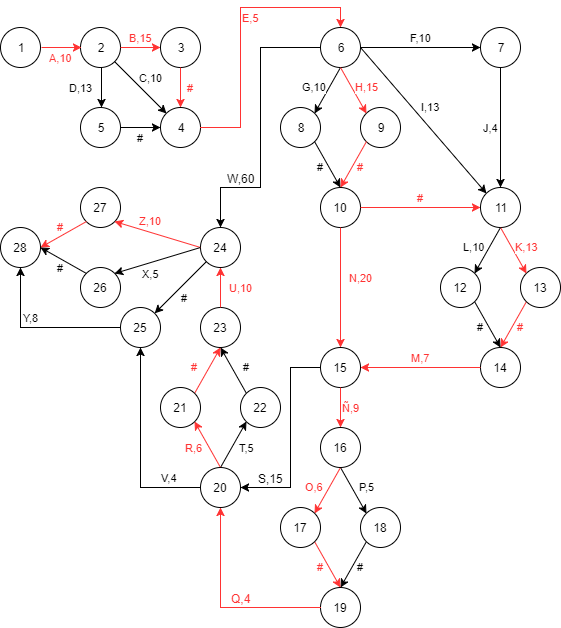
\includegraphics[scale=0.56]{imagenes/ruta_critica.png}
\caption{Red donde se destaca la ruta crítica.}
\end{figure}

Las actividades relacionas a las rutas críticas encontradas son:

$$A\longrightarrow{}B\longrightarrow{}E\longrightarrow{}H\longrightarrow{}K\longrightarrow{}M\longrightarrow{}\tilde{N}\longrightarrow{}O\longrightarrow{}Q\longrightarrow{}R\longrightarrow{}U\longrightarrow{}Z$$

$$A\longrightarrow{}B\longrightarrow{}E\longrightarrow{}H\longrightarrow{}N\longrightarrow{}\tilde{N}\longrightarrow{}O\longrightarrow{}Q\longrightarrow{}R\longrightarrow{}U\longrightarrow{}Z$$

El tiempo total de la atención de los empleados es de $110 [min]$.

\newpage
\section{Pregunta 2:}

Ahora se busca que la duración se reduzca en 12 minutos, es decir que el tiempo total sea de $98 [min]$. El modelo de programación lineal de \textit{crashing} para este proyecto se puede plantear de la siguiente manera:

\begin{itemize}
    \item Variables:
        $$x_i: \textrm{instante de ocurrencia del nodo }i;\forall{i}=1,...,28  $$
        $$y_j: \textrm{cantidad de tiempo a disminuir la actividad }j;\forall{j}=A,...,Z  $$
    \item Función objetivo:
        $$\min{z} = 3y_A + 1y_B + 5y_D + 1y_H + 4yI + 6y_K + 2y_M + 3y_N + 8y_{\tilde{N}} + 1y_O + 3y_R + 2y_S + 8y_U + 15y_W + 2y_Y + 5y_Z$$
    \item Restricciones:
        \begin{itemize}
            \item Inicio y fin de proyecto:
                $$x_1=0$$
                $$x_{28}\leq{98}$$
            \item Relaciones de precedencia entre las actividades que pueden ser aceleradas:
            \begin{multicols}{2}
                $$x_2\geq{x_1+10-y_A}$$
                $$x_3\geq{x_2+15-y_B}$$
                $$x_5\geq{x_2+13-y_D}$$
                $$x_9\geq{x_6+15-y_H}$$
                $$x_{11}\geq{x_6+13-y_I}$$
                $$x_{13}\geq{x_{11}+13-y_K}$$
                $$x_{15}\geq{x_{14}+7-y_M}$$
                $$x_{15}\geq{x_{10}+20-y_N}$$
                $$x_{16}\geq{x_{15}+9-y_{\tilde{N}}}$$
                $$x_{17}\geq{x_{16}+6-y_O}$$
                $$x_{21}\geq{x_{20}+6-y_R}$$
                $$x_{20}\geq{x_{15}+15-y_S}$$
                $$x_{24}\geq{x_{23}+10-y_U}$$
                $$x_{24}\geq{x_6+60-y_W}$$
                $$x_{28}\geq{x_{25}+8-y_Y}$$
                $$x_{27}\geq{x_{24}+10-y_Z}$$
                \end{multicols} 

            \item Relaciones de precedencia entre las demás actividades:
                \begin{multicols}{2}
                $$x_4\geq{x_2+10}$$
                $$x_6\geq{x_4+5}$$
                $$x_7\geq{x_6+10}$$
                $$x_8\geq{x_6+10}$$
                $$x_{11}\geq{x_7+4}$$
                $$x_{12}\geq{x_{11}+10}$$
                $$x_{18}\geq{x_{16}+5}$$
                $$x_{20}\geq{x_{19}+4}$$
                $$x_{22}\geq{x_{20}+5}$$
                $$x_{25}\geq{x_{20}+4}$$
                $$x_{26}\geq{x_{24}+5}$$
                \end{multicols} 
                
            \newpage
            \item Relaciones de precedencia entre actividades fantasmas:
                \begin{multicols}{3}
                $$x_4\geq{x_3}$$
                $$x_4\geq{x_5}$$
                $$x_{10}\geq{x_8}$$
                $$x_{10}\geq{x_9}$$
                $$x_{11}\geq{x_{10}}$$
                $$x_{14}\geq{x_{12}}$$
                $$x_{14}\geq{x_{13}}$$
                $$x_{19}\geq{x_{17}}$$
                $$x_{19}\geq{x_{18}}$$
                $$x_{23}\geq{x_{21}}$$
                $$x_{23}\geq{x_{22}}$$
                $$x_{25}\geq{x_{24}}$$
                $$x_{28}\geq{x_{26}}$$
                $$x_{28}\geq{x_{27}}$$
                \end{multicols}
            \item Cantidades máximas a disminuir:
                \begin{multicols}{3}
                $$y_A\leq{2}$$
                $$y_B\leq{3}$$
                $$y_D\leq{1}$$
                $$y_H\leq{5}$$
                $$y_I\leq{2}$$
                $$y_K\leq{3}$$
                $$y_M\leq{2}$$
                $$y_N\leq{10}$$
                $$y_{\tilde{N}}\leq{1}$$
                $$y_O\leq{2}$$
                $$y_R\leq{1}$$
                $$y_S\leq{4}$$
                $$y_U\leq{2}$$
                $$y_W\leq{5}$$
                $$y_Y\leq{3}$$
                $$y_Z\leq{2}$$
                \end{multicols}
            \item No negatividad:
                
                $$x_i,y_j\geq{0};\forall{i}=1,...,28;\forall{j}=A,...,Z$$
                
        \end{itemize}
\end{itemize}

\newpage
Para comenzar a acelerar las actividades, se debe seleccionar aquella que sea crítica y que posea el menor costo unitario. Esta condición la cumplen 3 actividades, siendo las B, H y O. Primero se acelerará a B, que será aumentado en 3 unidades a modo de resumen (ya que se mantiene en la ruta crítica en las dos primeras aceleraciones). Luego de esto, se suma un costo de 3 y los nuevos tiempos quedan de la siguiente forma:

\begin{table}[ht]
\centering
\begin{tabular}{|c|c|c|c|c|}
\hline
Act. & E min & E max & L min & L max \\ \hline
A    & 0     & 10    & 0     & 10    \\ \hline
B    & 10    & 22    & 11    & 23    \\ \hline
C    & 10    & 20    & 13    & 23    \\ \hline
D    & 10    & 23    & 10    & 23    \\ \hline
E    & 23    & 28    & 23    & 28    \\ \hline
F    & 28    & 38    & 29    & 39    \\ \hline
G    & 28    & 38    & 33    & 43    \\ \hline
H    & 28    & 43    & 28    & 43    \\ \hline
I    & 28    & 41    & 30    & 43    \\ \hline
J    & 38    & 42    & 39    & 43    \\ \hline
K    & 43    & 56    & 43    & 56    \\ \hline
L    & 43    & 53    & 46    & 56    \\ \hline
M    & 56    & 63    & 56    & 63    \\ \hline
N    & 43    & 63    & 43    & 63    \\ \hline
Ñ    & 63    & 72    & 63    & 72    \\ \hline
O    & 72    & 78    & 72    & 78    \\ \hline
P    & 72    & 77    & 73    & 78    \\ \hline
Q    & 78    & 82    & 78    & 82    \\ \hline
R    & 82    & 88    & 82    & 88    \\ \hline
S    & 63    & 78    & 67    & 82    \\ \hline
T    & 82    & 87    & 83    & 88    \\ \hline
U    & 88    & 98    & 88    & 98    \\ \hline
V    & 82    & 86    & 96    & 100   \\ \hline
W    & 28    & 88    & 38    & 98    \\ \hline
X    & 98    & 103   & 103   & 108   \\ \hline
Y    & 98    & 106   & 100   & 108   \\ \hline
Z    & 98    & 108   & 98    & 108   \\ \hline
\end{tabular}
\end{table}

Se logra apreciar que luego de esta optimización, la actividad D pasa a ser parte de la ruta crítica y que la actividad B deja de ser parte de esta. Luego, la ruta se ve de la siguiente forma:

$$A\longrightarrow{}D\longrightarrow{}E\longrightarrow{}H\longrightarrow{}K\longrightarrow{}M\longrightarrow{}\tilde{N}\longrightarrow{}O\longrightarrow{}Q\longrightarrow{}R\longrightarrow{}U\longrightarrow{}Z$$

$$A\longrightarrow{}D\longrightarrow{}E\longrightarrow{}H\longrightarrow{}N\longrightarrow{}\tilde{N}\longrightarrow{}O\longrightarrow{}Q\longrightarrow{}R\longrightarrow{}U\longrightarrow{}Z$$

\newpage
Para ahorrar espacio, las iteraciones se pueden resumir como lo siguiente:

\begin{table}[ht]
\centering
\begin{tabular}{|c|c|c|}
\hline
Actividad & Aceleración & Costo \\ \hline
A         & 2           & 6     \\ \hline
B         & 3           & 3     \\ \hline
C         & 0           & 0     \\ \hline
D         & 1           & 5     \\ \hline
E         & 0           & 0     \\ \hline
F         & 0           & 0     \\ \hline
G         & 0           & 0     \\ \hline
H         & 3           & 3     \\ \hline
I         & 0           & 0     \\ \hline
J         & 0           & 0     \\ \hline
K         & 0           & 0     \\ \hline
L         & 0           & 0     \\ \hline
M         & 2           & 4     \\ \hline
N         & 0           & 0     \\ \hline
Ñ         & 0           & 0     \\ \hline
O         & 1           & 1     \\ \hline
P         & 0           & 0     \\ \hline
Q         & 0           & 0     \\ \hline
R         & 1           & 3     \\ \hline
S         & 0           & 0     \\ \hline
T         & 0           & 0     \\ \hline
U         & 0           & 0     \\ \hline
V         & 0           & 0     \\ \hline
W         & 0           & 0     \\ \hline
X         & 0           & 0     \\ \hline
Y         & 0           & 0     \\ \hline
Z         & 2           & 10    \\ \hline
\end{tabular}
\end{table}

\newpage

Finalmente, se obtiene un costo de $35 [\$]$ para acelerar en 12 unidades. La nueva red y ruta crítica es la siguiente:

\begin{table}[ht]
\centering
\begin{tabular}{|c|c|c|c|c|}
\hline
Act. & E min & E max & L min & L max \\ \hline
A    & 0     & 8     & 0     & 8     \\ \hline
B    & 8     & 20    & 8     & 20    \\ \hline
C    & 8     & 18    & 10    & 20    \\ \hline
D    & 8     & 20    & 8     & 20    \\ \hline
E    & 20    & 25    & 20    & 25    \\ \hline
F    & 25    & 35    & 25    & 35    \\ \hline
G    & 25    & 35    & 29    & 39    \\ \hline
H    & 25    & 37    & 27    & 39    \\ \hline
I    & 25    & 38    & 26    & 39    \\ \hline
J    & 35    & 39    & 35    & 39    \\ \hline
K    & 39    & 52    & 39    & 52    \\ \hline
L    & 39    & 49    & 42    & 52    \\ \hline
M    & 52    & 57    & 52    & 57    \\ \hline
N    & 37    & 57    & 37    & 57    \\ \hline
Ñ    & 57    & 66    & 57    & 66    \\ \hline
O    & 66    & 71    & 66    & 71    \\ \hline
P    & 66    & 71    & 66    & 71    \\ \hline
Q    & 71    & 75    & 71    & 75    \\ \hline
R    & 75    & 80    & 75    & 80    \\ \hline
S    & 57    & 72    & 60    & 75    \\ \hline
T    & 75    & 80    & 75    & 80    \\ \hline
U    & 80    & 90    & 80    & 90    \\ \hline
V    & 75    & 79    & 86    & 90    \\ \hline
W    & 25    & 85    & 30    & 90    \\ \hline
X    & 90    & 95    & 93    & 98    \\ \hline
Y    & 90    & 98    & 90    & 98    \\ \hline
Z    & 90    & 98    & 90    & 98    \\ \hline
\end{tabular}
\end{table}

$$Ruta critica = A - B - D - E - F - J - K - M - N - \tilde{N} - O - P - Q - R - T - U - Y - Z$$

\end{document}
